\subsection{Karp-Luby Algorithm in the Continuous}


The number  of condition atoms in a  given row  is linear in  the query
complexity;  every renaming operator  adds a  fixed number  of condition
atom  columns to the  table, while  a join  simply merges  the condition
columns  of both  input tables.   Thus, the  size of  each conjunctive
clause is fixed with respect to the amount of input data and typically
relatively small.   However, there is no  such bound on  the number of
conjunctive  clauses  in a DNF.   Thus,  while  it  is
reasonable for  PIP to perform conjunctive integration  in memory, PIP
must use the disk to store intermediate state when computing integrals
of DNF formulas.

Two techniques may  be used to estimate the general  integral of a set
of conjunctive clauses of atoms.  Under naive Monte Carlo integration,
PIP first generates a set of samples and performs a linear scan of the
conjunctive clauses to determine how many samples are true in at least
one conjunctive clause.  The  number of samples required is determined
both by  the scale  of the answer  and the desired  precision.  Though
straightforward,  this  approach is  inefficient  if  the value  being
computed is small.

An  alternative approach  is a  Karp-Luby style  estimator, as
used  in the discrete case in \cite{RDS07, KO2008}.   This  approach first  computes  the
independent probability of each  conjunctive clause.  The sum of these
probabilities, termed the bag sum, is computed and stored.  Though the
bag sum is  related to the integral, the two are  not equal unless the
conjunctive clauses  are all mutually exclusive.  If  there is overlap
between clauses,  the bag sum will  exceed the value  of the integral.
The Karp-Luby estimator computes  this overlap, generating an estimate
of the ratio of the integral to the bag sum.

After computing the  bag probabilities and the bag  sum, the Karp-Luby
estimator  generates  samples  for  each clause,  constrained  to  the
subspace  it defines.   Each clause  is used  to produce  a  number of
samples  proportional  to  its  contribution  to  the  bag  sum.   The
generated samples  are compared agaainst  all clauses.  The  number of
clauses that  satisfy a given sample  are counted, and  the average of
the inverse of the counts is the ratio of the integral to the bag sum.
This value is multiplied by the  bag sum to produce an estimate of the
integral.  This algorithm is summarized in Figure
\ref{fig:klestimator}


\begin{figure}
\begin{center}
\begin{enumerate}
\item Perform a linear scan of the clauses $C$ of the disjunction, computing $P[\vec{\phi_C}]$.  As part of the same scan, compute $bag\_sum = \sum_C P[\vec{\phi_C}]$.  
\item Perform another linear scan, this time generating $total\_samples \cdot \frac{P[clause]}{bag\_sum}$ samples $\vec{S}$. 
\item Perform a final linear scan over $\vec{C} \bowtie \vec{S}$.  Compute the array $Sat[S] = \sum_C \chi_{\vec{\phi_C}}(S)$
\item The average value $\frac{1}{|\vec{S}|} \sum_{S}\frac{1}{Sat[S]}$ is an estimator for the ratio of the integral to the bag sum. 
\end{enumerate}
\caption{The Karp-Luby Estimator}
\label{fig:klestimator}
\end{center}
\end{figure}


There  is an  evident  tradeoff between  these  two processes.   naive
sampling is  faster when constrained  sampling cannot  be efficiently
performed.   However,  even  in  this case,  the  Karp-Luby  estimator
provides a more consistent precision; it generates a consistent number
of ``useful'' samples, even though  doing so is more expensive.  These
processes are summarized in Figure \ref{fig:integration}.


\begin{figure}
\begin{center}
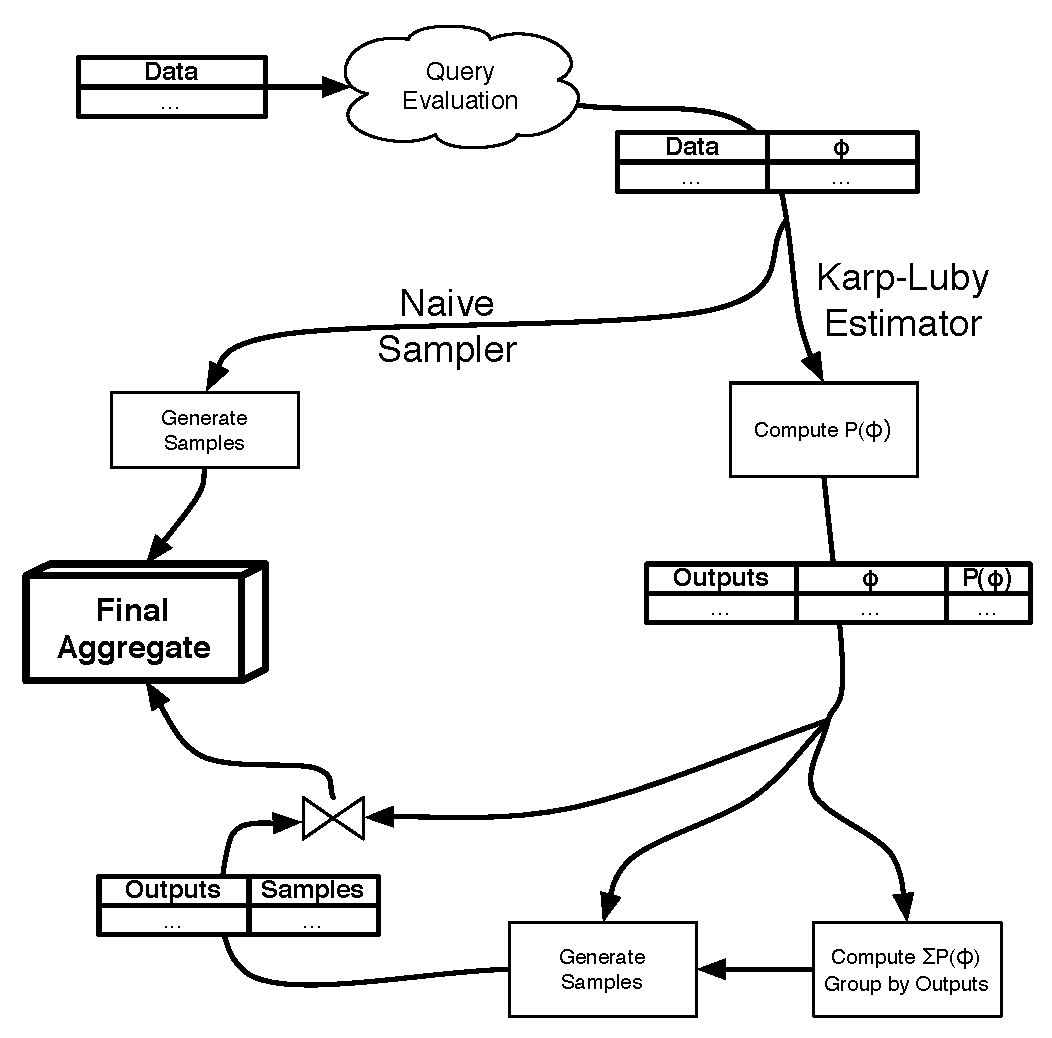
\includegraphics[width=3.2in]{graphics/sampling_flowchart.pdf}
\end{center}

\vspace{-5mm}

\caption{\textbf{General Integration}}
\label{fig:integration}
\end{figure}


